
%  Verwendete Plattform /Software (Installationshinweise, Versionen)
% Schnittstellenbeschreibung des Web Services (WSDL/WADL/Swagger, …​)
% Umsetzung, Technologien, Sicherheitskonzepte, API

\section{Technologien}


\subsection{Architektur}

%Beschriebender Text?

\begin{figure}[H]
	\hspace{-1.5cm}
	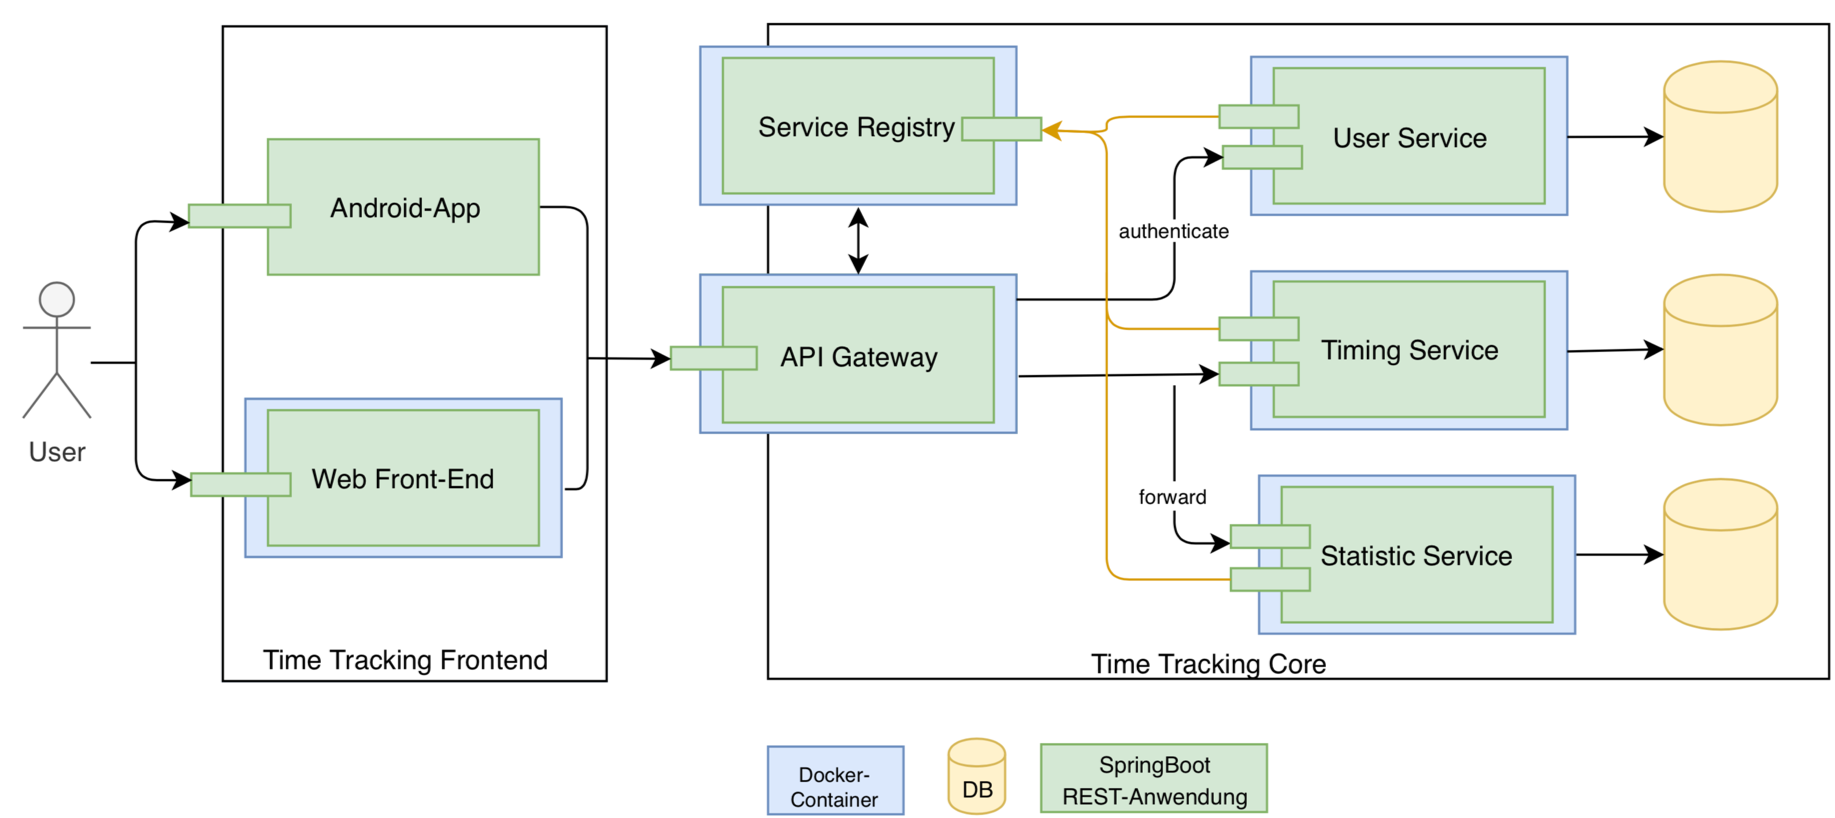
\includegraphics[width=1.15\linewidth]{SCC_Architecture-99final.png}
	\caption{Architektur von TimeTracker}
	\label{fig:Architektur}
\end{figure}

Anmerkung: Die Andoid-App wurde nicht im Rahmen der Lehrveranstaltung fertig gestellt und ist somit noch ausstehend. 

\subsection{Übersicht verwendeter Technologien}
% Tabelle 
\begin{table}[H] 
	% \small
	\centering
	\caption{Technologien}
	\begin{tabularx}{\textwidth}{l|c|X}
		\textbf{Name} & \textbf{Version} & \textbf{Verwendung} \\
		\hline
		Java & bla & bla \\
		Mavent & 3.1.0 & bla \\
		Spring boot & bla & bla \\
		MySQL & bla & bla \\
		Netflix Zuul & bla & bla \\
		Netflix Eureka & bla & bla \\
		JSON & bla & bla \\
		REST & bla & bla \\
		React & bla & bla \\
		single.spa & bla & bla \\
		OpenAPI + Swagger & bla & bla \\
		Postman & bla & bla \\
		Docker & bla & bla \\
	\end{tabularx}
	\label{tab:Technologien}
\end{table}

\subsection{Umsetzung}
% benötigt? 

\subsection{Schnittstellenbeschreibung}
- von swagger? 


\subsection{Sicherheit}
JSON Web Token   

HTTPS

